\section{Schedule}

The detector installation planning hinges on the date that the \dword{jpo} is permitted to begin work underground. According to the \dword{dune} \dword{cf} schedule, the \dword{jpo} receives the \dword{aup} for  the north cavern and \dword{cuc} in \cucbenocc{}.  The  \dword{sdwf} will be in place approximately six months before the warm structure installation begins, i.e., in spring 2022. Building the schedule for the \dword{detmodule} \#1 installation after \dword{aup} is  complicated and depends on many entities including \dword{cf}, \dword{lbnf}, and \dword{sdsta}.  The maximum number of people allowed underground is 144, which is the number of people that can be evacuated in one hour.  This places a hard bound on how much work can be performed underground at any time and is particularly critical during the excavation of the third cavern when \dword{cf} is still active. Figure \ref{fig:Overview-of-SinglePhase-Schedule} shows the main activities for the \dword{detmodule} \#1 installation and  the high-level milestones are shown in Table~\ref{tab:sp-iic-sched}.

The cost, schedule, and labor estimates are based on two \SI{10}{hour} shifts per day, four days a week (Monday through Thursday). Work efficiency should be a maximum of \SI{70}{\%}.  The cage ride, shift meetings, lunch, coffee breaks, and cleanroom gowning takes %up approximately 2-3 
up to three hours per day. Some low level of effort is planned on Friday, Saturday, and Sunday to monitor the \coldbox{}es and take data. 

\begin{dunetable}
[\dshort{sp} Installation, Integration, and Commissioning Milestones]
{p{0.65\textwidth}p{0.25\textwidth}}
{tab:sp-iic-sched}
{\dword{sp} Installation, Integration, and Commissioning Schedule}   
Milestone & Date (Month YYYY)   \\ \toprowrule

Ash River phase 0 complete &  March 2020    \\ \colhline
\rowcolor{dunepeach} Start of \dword{pdsp}-II installation& \startpduneiispinstall      \\ \colhline
Ash River phase 1 complete & June 2021     \\ \colhline
 \dword{cuc} \dword{prr} & July 2021     \\ \colhline
Installation Preliminary Design Review & August 2021     \\ \colhline

\rowcolor{dunepeach} Start of \dword{pddp}-II installation& \startpduneiidpinstall      \\ \colhline
\rowcolor{dunepeach}South Dakota Logistics Warehouse available& \sdlwavailable      \\ \colhline
Begin procurement of \dword{cuc} equipment  &   April 2022   \\ \colhline

Ash River phase 2 complete &  July 2022    \\ \colhline
Installation \dword{prr} &  August 2022    \\ \colhline
Start production of installation infrastructure Detector \#1 & August 2022     \\ \colhline
Installation Final Design Review  & September 2022     \\ \colhline
\rowcolor{dunepeach}Beneficial occupancy of cavern 1 and \dword{cuc}& \cucbenocc      \\ \colhline
Start construction warm structure cryostat \#1   & October 2022     \\ \colhline
Start outfitting of \dword{cuc}  &  October 2022    \\ \colhline

\rowcolor{dunepeach} \dword{cuc} counting room accessible& \accesscuccountrm      \\ \colhline
Start installation of  cold structure Cryostat\#1 &  August 2023    \\ \colhline
Start installing Detector\#1 infrastructure  &  August 2023    \\ \colhline
\rowcolor{dunepeach}Top of \dword{detmodule} \#1 cryostat accessible& \accesstopfirstcryo      \\ \colhline
Begin Detector\#1 installation   &   June 2024   \\ \colhline

\rowcolor{dunepeach}Start of \dword{detmodule} \#1 TPC installation& \startfirsttpcinstall      \\ \colhline
\rowcolor{dunepeach}Top of \dword{detmodule} \#2 accessible& \accesstopsecondcryo      \\ \colhline
\rowcolor{dunepeach}End of \dword{detmodule} \#1 TPC installation& \firsttpcinstallend      \\ \colhline
TCO detector \#1 closed  &  July 2025    \\ \colhline
Start of cryogenic operation for detector \#1  &  August 2025    \\ \colhline
 \rowcolor{dunepeach}Start of \dword{detmodule} \#2 TPC installation& \startsecondtpcinstall      \\ \colhline
\rowcolor{dunepeach}End of \dword{detmodule} \#2 TPC installation& \secondtpcinstallend      \\ \colhline
Start of  detector\#1 commissioning  & January 2027     \\ \colhline                        \\
\end{dunetable}



\begin{dunefigure}[Overview of the single-phase schedule]
{fig:Overview-of-SinglePhase-Schedule}
{Schedule Overview of the \dword{sp} \dword{detmodule} \#1}                
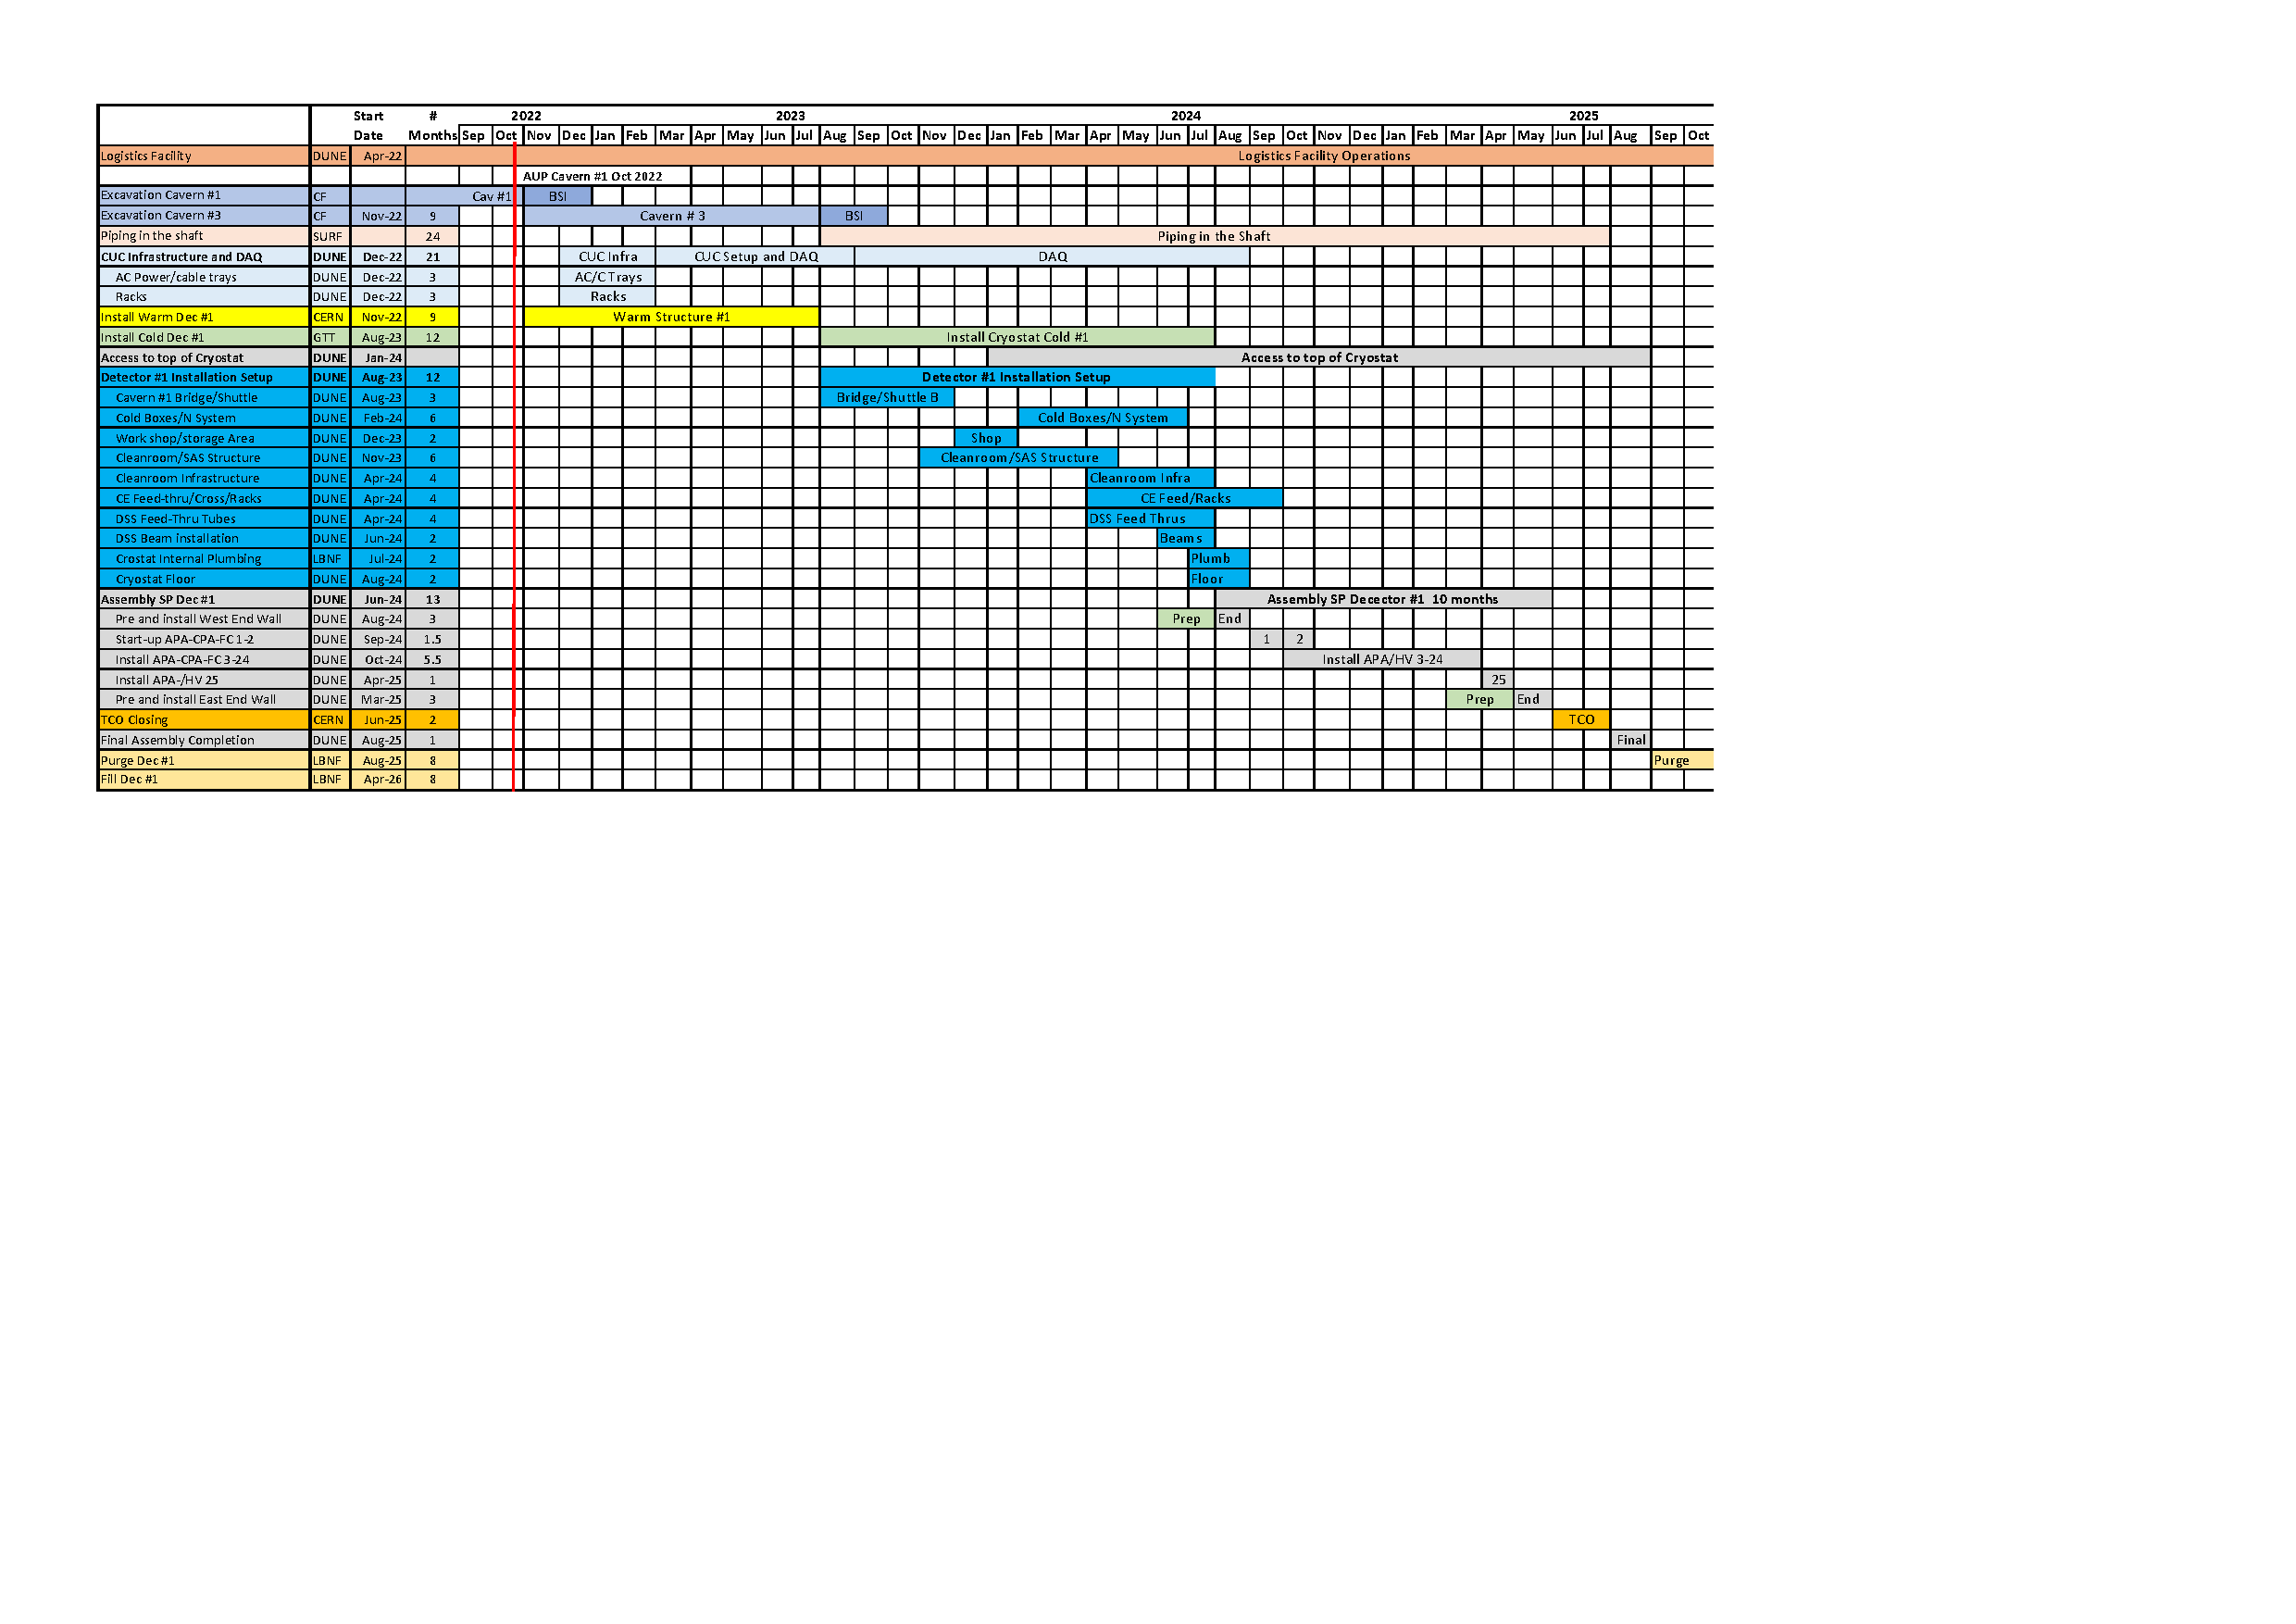
\includegraphics[angle=90, width=0.55\textwidth]
{Overview-of-SinglePhase-Schedule}
\end{dunefigure}



%As described earlier there are  three basic schedule phases for Detector 1 installation:
We have defined three schedule phases for installation of the first \dword{spmod}:

\begin{itemize}
%    \item {\bf \dword{cuc} Installation Phase:}
%    This period, which is described in detail in section \ref{sec:fdsp-tc-inst-CUC}, can start once \dword{aup} has been received for the north cavern and the \dword{cuc}. This is also the same time that excavation of the south cavern and installation of the warm structure by \dword{lbnf} begins. As no more than 144 \dwords{fte} will be allowed underground at a time,  access to the underground area will be minimal during this period for \dword{dune} personnel.  Work in this period is limited to work inside the \dword{cuc} and surface dataroom. Installing the basic rack infrastructure in the datarooms will take an estimated three months, and then installation and testing of the \dword{daq} will continue over the next 12 month period. The \dword{daq} is needed at the start of detector installation.  
   \item {\bf \dword{cuc} Installation Phase:}
    This period,described in detail in Section~\ref{sec:fdsp-tc-inst-CUC}, starts once \dword{aup} has been received for the north cavern and the \dword{cuc}. This is the same time that excavation of the south cavern and installation of the warm structure by \dword{lbnf} begins. Since the \dwords{fte} underground is limited to 144 at a time, access will be minimal for \dword{dune} personnel and their work will only take place inside the \dword{cuc} and surface dataroom. Installing the basic rack infrastructure in the dataroom will take an estimated three months. Installation and testing of the \dword{daq} (required at the start of detector installation) will continue over the next 12 month period. Ten DAQ workers are planned on each shift in this period.
     
    
    
    %\item {\bf Installation Setup Phase:} This phase,  described in detail in section \ref{sec:fdsp-tc-inst-setup}, is when the majority of the infrastructure is installed. This is a critical training period, so getting lead-workers, riggers, and equipment operators familiar with the tasks is a priority, and adjusting crews to ensure balanced teams.   Before this phase, the \dword{dune} trial assembly equipment at Ash River will be used to begin the training process. This is a more difficult phase to schedule and may require frequent adjustment, with multiple projects going forward at once. Immediately after the cryostat warm structure is complete the north-south bridge is constructed. Following this the bridge crane under the bridge can be installed. A few months after the cryostat warm structure is complete the \dword{cf} work is also complete and the 80 of 144 underground workers which \dword{cf} had been using are available to the \dword{jpo}, working two 10 hour shifts per day begins, and the \dword{uit} team doubles in size.  Peripheral work on the cleanroom structure and assembly towers can then begin as they will not take up too much floor space. Once the  cryostat cold structure is approximately six months into the installation schedule most of the foam has been installed and floor space becomes available in the north cavern. The \coldbox construction must begin immediately at this point because the welding takes approximately six months. In parallel, the machine shop area can be set up. As the membrane installation nears completion the walls of the cleanroom can be installed and the remaining equipment. 
    
   % Installation of the \dword{dss} could begin during the final installation stages of the cryostat cold structure because they both require full-height scaffolding for the welding on the top of the cryostat. The \dword{protodune} \dword{dss} was installed this way. This requires a crew on top of the cryostat installing the \dword{dss} support feedhroughs from the top, as shown in Figure~\ref{fig:install-dss-feedthru}.  The details have not yet been worked out with the contractor, so work may be done in stages. 
   
    \item {\bf Installation Setup Phase:}  Described in detail in section \ref{sec:fdsp-tc-inst-setup}, this period includes installation of  the majority of the infrastructure. The setup phase is a critical training period, so getting lead-workers, riggers, and equipment operators familiar with the tasks is a priority, as is  adjusting the crews to ensure balanced teams. The training process will have begun already at Ash River. 
    There are many parallel underground activities planned in this phase making it a difficult phase to schedule and frequent schedule adjustments may be required. Immediately after the cryostat warm structure is complete the north-south bridge is constructed. Following this the bridge crane under the bridge can be installed. A few months after the cryostat warm structure is complete the \dword{cf} work will also complete, and 80 of the 144 underground workers will become available to the \dword{jpo} and the \dword{uit} team doubles in size. The \dword{jpo} will start two \SI{10}{hour} shifts per day.  Due to space constraints, peripheral work only on the cleanroom structure and assembly towers can begin. Once the  cryostat cold structure is approximately six months into its installation schedule, most of the foam will have been installed and floor space becomes available in the north cavern. The \coldbox construction must begin immediately at this point because the welding takes approximately six months. In parallel, the machine shop area can be set up. As the membrane installation nears completion, the walls of the cleanroom can be installed as can the remaining equipment. 
    
    Installation of the \dword{dss} could begin during the final installation stages of the cryostat cold structure because they both require full-height scaffolding for the welding on the top of the cryostat. The \dword{pdsp} \dword{dss} was installed this way. This requires a crew on top of the cryostat installing the \dword{dss} support feedthroughs from the top, as shown in Figure~\ref{fig:install-dss-feedthru}.  The details have not yet been worked out with the contractor, and work may be done in stages.

    %\item {\bf Detector Installation Phase:} The final detector installation phase begins with an operational readiness review to check that all documentation and procedures are in place. After the east endwalls are installed, a start-up period of 1.5 months begins for the first two rows of \dword{tpc} components.  To meet this schedule, three assembly lines, three coldboxes, and separate crews in the cryostat, all working in parallel are needed.  It will take 5.5 months to install rows 3-24 and about 1 month for row 25. Closing the \dword{tco} will take approximately two months for the cryostat cold structure contractor. During this time, there is no access to the cryostat.  Once this is completed, the final instrumentation is completed, and the purge can begin. 
    \item {\bf Detector Installation Phase:} The final detector installation phase begins with an \dword{orr} to check that all documentation and procedures are in place. After the east \dwords{ewfc} are installed, a start-up period of 1.5 months begins for the first two rows of \dword{tpc} components.  To meet this schedule, three assembly lines, three \coldbox{}es, and separate crews in the cryostat, all working in parallel, are needed.  It will take 5.5 months to install rows 3 through 24 and about one month for row 25. Closing the \dword{tco} will take approximately two months for the cryostat cold structure contractor; during this time, there is no access to the cryostat.  Once this is completed, the final instrumentation is completed, and the purge can begin. During this period up to 50 people will be working in the cleanroom and cryostat.
    
\end{itemize}

The total time to install the detector including the time for the setup phase is two years. Coincidentally this was also roughly the time needed to install Minos or \dword{nova}.

  




% clear the figure buffer before starting the next section
%\clearpage


%\subsection{Detector Commissioning Phase}
%\label{sec:fdsp-tc-inst-comiss}

%\fixme{seems like this could use its own section right after detector installation and before cost and schedule. Then just put a summary here. So that's what I did 4/18. Please work on the summary below that I started!  anne}

%The detector commissioning phase covers the period after the \dword{tco} is closed until \dword{dune} operations begin. It is expected to take \num{12} months to complete the \dword{lar} fill. 